%% =============================================================================
%% Mathematische Grundlagen - Grundbegriffe
%% Kapitel 06 - Abbildungen und Funktionen
%% Autor: Andreas Zeh-Marschke
%% Datum: 2025-03-31
%% =============================================================================

\chapter{Abbildungen und Funktionen}
\label{cha:Gdl-K06-Abbildungen}

%% -----------------------------------------------------------------------------
%\begin{unit}
Eine spezielle Relation ist die Abbildung. Auf Grund der Wichtigkeit für den 
gesamten Bereich der Mathematik, werden Abbildungen genauer betrachtet. Nach 
der Definition von \textbf{Abbildungen} (Abschnitt 
\ref{sec:Abbildungen:Definition}) werden \textbf{Eigenschaften} von
Abbildungen (siehe Abschnitt \ref{sec:Abbildungen:Eigenschaften}) erläutert. 
Im Abschnitt \ref{sec:Abbildungen:Mengen von Abbildungen} werden kurz Mengen 
von Abbildungen betrachtet.
%\end{unit}

%%------------------------------------------------------------------------------
%% Abschnitt: Definition von Abbildungen
%%------------------------------------------------------------------------------
\section{Definition von Abbildungen}
\label{sec:Abbildungen:Definition}

%% -----------------------------------------------------------------------------
\begin{Unit}[Definition Abbildung]
Gleich die einfache Definition einer Abbildung.

\begin{Definition}
  Es seien $X$ und $Y$ zwei beliebige, nicht leere Mengen und $f \subseteq X 
  \times Y$ eine Vorschrift, die jedem Element von $X$ genau ein Element aus 
  $Y$ zuordnet:
  \begin{align}
    \forall x \in X\ \exists^1 y \in Y\ : (x, y) \in f \ .
  \end{align}
  Das Tripel $(f,X,Y)$ oder kurz $f$ heißt \Begriff{Abbildung} von $X$ nach 
  $Y$. Dafür wird auch 
  \begin{align}
    f:X \rightarrow Y\ ,\ x \mapsto f(x) = y 
  \end{align}
  geschrieben.
  Die Menge $X$ heißt der \Begriff{Definitionsbereich} von $f$. Die Menge 
  $Y$ heißt der \Begriff{Wertebereich} von $f$. Die Menge 
  \begin{align}
    f(X) := \{y \in Y \mid \exists x \in X: f(x) = y\}
  \end{align} 
  heißt \Begriff{Bild} von $f$, und die Menge 
  \begin{align}
    graph(f) := \{(x, f(x)) \mid x \in X\}
  \end{align} heißt \Begriff{Graph} von $f$.
\end{Definition}
\Translation{Abbildung}{mapping}
\Translation{Definitionsbereich}{domain}
\Translation{Wertebereich}{codomain}
\Translation{Graph}{graph}

\begin{figure}[htbp]
\begin{center}
  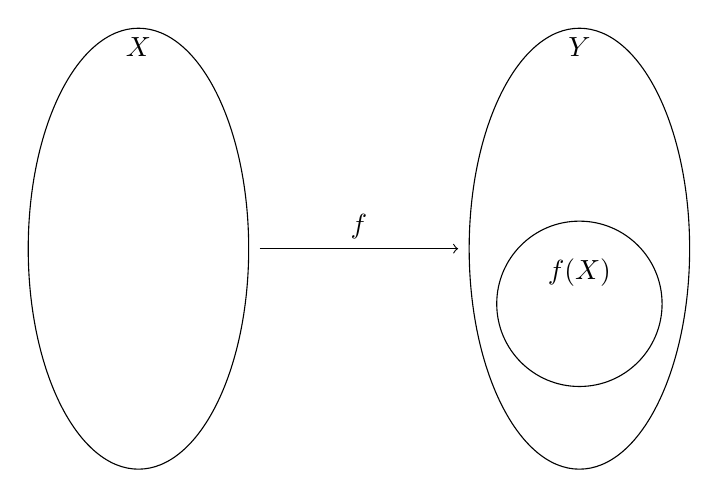
\begin{tikzpicture}[scale=0.7]
    \draw (-4.0,0.0) ellipse (2.0 and 4.0);
    \draw (-4.0,4.0) node[below]{$X$};
    \draw (4.0,0.0) ellipse (2.0 and 4.0);
    \draw (4.0,4.0) node[below]{$Y$};
    \draw (4.0,-1.0) circle (1.5);
    \draw (4.0,0.0) node[below]{$f(X)$};
    \draw[->] (-1.8,0.0) -- (1.8,0.0);
    \draw (0.0,0.0) node[above]{$f$};
  \end{tikzpicture}
  \caption{Abbildung}
  \label{abb:abb:Abbildung}
\end{center}
\end{figure}

Auf Grund der Eigenschaft $f \subseteq X \times Y$ ist $f$ eine Relation von 
$X \times Y$. Die zusätzliche Eigenschaft bedeutet, dass es für jedes Element 
von $x \in X$ genau ein Element $y \in Y$ gibt, so dass $(x,y) \in f$ ist. Es 
wird zwischen der Abbildung $f$ und dem Wert $f(x)$ der Abbildung $f$ an der 
Stelle $x$ unterschieden. In der Abbildung \ref{abb:abb:Abbildung} ist die 
Abbildung grafisch dargestellt.

Das Bild von $f$ ist eine Teilmenge von $Y$ $(f(X) \subseteq Y)$, der Graph 
von $f$ ist eine Teilmenge des kartesischen Produktes von $X$ und $Y$ 
$(graph(f) \subseteq X \times Y)$.
\end{Unit} 

%% -----------------------------------------------------------------------------
\begin{Unit}[Definition Gleichheit]
Wann sind zwei Abbildung gleich?

\begin{Definition}
Zwei Abbildungen $f: X \rightarrow Y$ und $g: X \rightarrow Y$ heißen
\Begriff{gleich}, wenn $f(x) = g(x)$ für alle $x \in X$ gilt.
\begin{align}
   f = g :\Leftrightarrow \forall x \in X: f(x) = g(x) \ .
\end{align}
\end{Definition}
\Translation{Gleichheit}{equality}

Hierbei ist auch wichtig, dass die Definitionsbereiche und die Wertebereiche
identisch sind.
\end{Unit} 

%% -----------------------------------------------------------------------------
\begin{Unit}[Beispiel] 
Die Abbildung, die einer natürlichen Zahl $n$ seinen Nachfolger zuordnet.
\begin{align}
  f: \NN \rightarrow \NN,\ n \mapsto f(n) = n + 1
\end{align}
$f(\NN) = \NN \backslash \{1\}$
\end{Unit}

%% -----------------------------------------------------------------------------
\begin{Unit}[Beispiel] 
Die Abbildung, die jeder natürlichen Zahl sein Doppeltes zuordnet.
\begin{align}
  f: \NN \rightarrow \NN,\ n \mapsto f(n) = 2n
\end{align}
$f(\NN) = \{2, 4, 6, 8, \ldots \}$
\end{Unit}

%% -----------------------------------------------------------------------------
\begin{Unit}[Beispiel] 
Die Abbildung, die jeder ganzen Zahl $z$ seinen Nachfolger zuordnet.
\begin{align}
  f: \ZZ \rightarrow \ZZ,\ z \mapsto f(z) = z + 1
\end{align}
$f(\ZZ) = \ZZ$
\end{Unit}

%% -----------------------------------------------------------------------------
\begin{Unit}[Beispiel] 
Die Abbildung, die einer geraden natürlichen Zahl den halben Wert zuordnet.
Den ungeraden natürlichen Zahlen wird eine negative Zahl zugeordnet.
\begin{align}
  f: \NN \rightarrow \ZZ, n \mapsto f(n) := 
  \begin{cases} 
    n/2      & \text{ falls }n{\ gerade } \\ 
    -(n-1)/2 & \text{ falls }n{\ ungerade } \ .
  \end{cases}
\end{align}
Es ist eine Abbildung von den natürlichen Zahlen in die Menge der ganzen 
Zahlen. Hierbei gibt es für jede ganze Zahl $z$ eine natürliche Zahl $n$, so
dass $f(n) = z$ ist. Somit gilt hier $f(\NN) = \ZZ$.
\end{Unit}

%% -----------------------------------------------------------------------------
\begin{Unit}[Beispiel] 
Die Abbildung, die jeder reellen Zahl das Quadrat der Zahl zuordnet.
\begin{align}
  f: \RR \rightarrow \RR, x \mapsto f(x) = x^2 \ .
\end{align}
Der Wertebereich sind die positiven reellen Zahlen, inklusive der $0$, es 
gilt also $f(\RR) = \RR^+_0$.
\end{Unit}

%% -----------------------------------------------------------------------------
\begin{Unit}[Beispiel] 
  \begin{align}
    f: \RR \rightarrow \RR, x \mapsto f(x) = \sqrt{x}
  \end{align}
  ist keine Abbildung, da nicht jedem $x \in \RR$ genau ein Wert zugewiesen 
  werden kann, da zum Einem die Wurzel von negativen Zahlen in $\RR$ nicht 
  definiert ist, und zum Anderen für positive Werte von $x \in \RR$ die 
  Wurzel zwei Lösungen hat, die positive und die negative Wurzel. Wird die 
  Vorschrift auf positive Werte eingeschränkt: $f:\RR^+_0 \rightarrow 
  \RR^+_0, x \mapsto f(x) = +\sqrt{x}$ dann entsteht eine Abbildung, mit 
  $f(\RR^+_0) = \RR^+_0$.
  
  Es ist die Regel, dass die Wurzel aus einer Zahl immer positiv ist. Daher
  gilt $\sqrt{x^2} = |x|$.
\end{Unit}

%% -----------------------------------------------------------------------------
\begin{Unit}[Beispiel] 
  Es sei $X$ eine Menge von Gütern, durch $u: X \rightarrow \RR, x \mapsto 
  u(x)$, wobei $u(x)$ der Nutzen des Gutes $x$ darstellt, wird eine Abbildung 
  definiert.
\end{Unit}

%% -----------------------------------------------------------------------------
\begin{Unit}[Beispiel]  
  Es sei $M$ eine (endliche) Menge und $\mathcal{P}(M)$ die Potenzmenge von 
  $M$, dann wird durch
  \begin{align}
    f: \mathcal{P}(M) \rightarrow \NN_0, T \mapsto f(T) := |T|
  \end{align}
  eine Abbildung definiert. Die Abbildung ordnet jeder Menge die Anzahl der 
  Elemente der Menge zu.
\end{Unit}

%% -----------------------------------------------------------------------------
\begin{Unit}[Definition Bild, Urbild]
Auch für Teilmengen $A \subseteq X$ und $B \subseteq Y$ können wir die Wirkung 
einer Abbildung $f:X \rightarrow Y$ betrachten.

\begin{Definition}
  Es sei $f: X \rightarrow Y$ eine Abbildung. Für $A \subseteq X$ heißt die 
  Menge
  \begin{align}
    f(A) := \{y \in Y \mid \exists x \in A : f(x) = y\}
  \end{align}
  das \Begriff{Bild} von $A$ unter $f$. Für $B \subseteq Y$ heißt die Menge
  \begin{align}
    f^{-1}(B) := \{x \in X \mid f(x) \in B\}
  \end{align}
  das \Begriff{Urbild} von $B$ unter $f$. Für ein $y \in Y$ wird
  \begin{align}
    f^{-1}(y) := \{x \in X \mid f(x) = y\} = f^{-1}(\{y\})
  \end{align}
  gesetzt.
\end{Definition}
\Translation{Bild}{image}
\Translation{Urbild}{preimage}

In den beiden Abbildungen \ref{abb:abb:Bild} und \ref{abb:abb:Urbild} sind 
die Beziehungen grafisch dargestellt.

\begin{figure}[htbp]
\begin{center}
  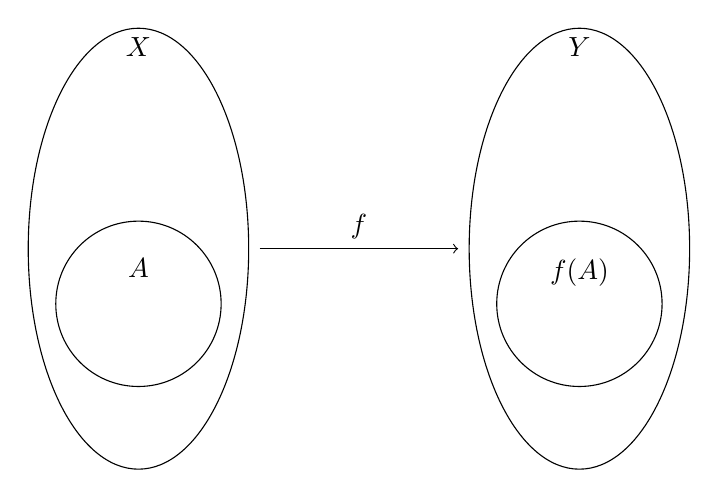
\begin{tikzpicture}[scale=0.7]
    \draw (-4.0,0.0) ellipse (2.0 and 4.0);
    \draw (-4.0,4.0) node[below]{$X$};
    \draw (-4.0,-1.0) circle (1.5);
    \draw (-4.0,0.0) node[below]{$A$};
    \draw (4.0,0.0) ellipse (2.0 and 4.0);
    \draw (4.0,4.0) node[below]{$Y$};
    \draw (4.0,-1.0) circle (1.5);
    \draw (4.0,0.0) node[below]{$f(A)$};
    \draw[->] (-1.8,0.0) -- (1.8,0.0);
    \draw (0.0,0.0) node[above]{$f$};
  \end{tikzpicture}
  \caption{Bild}
  \label{abb:abb:Bild}
\end{center}
\end{figure}

\begin{figure}[htbp]
\begin{center}
  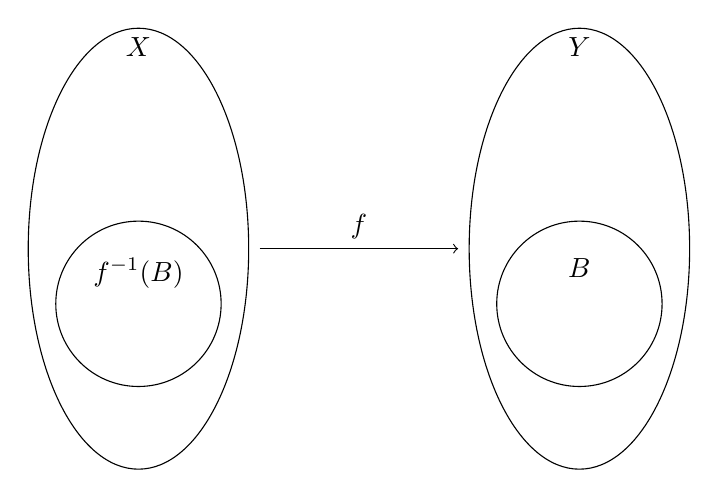
\begin{tikzpicture}[scale=0.7]
    \draw (-4.0,0.0) ellipse (2.0 and 4.0);
    \draw (-4.0,4.0) node[below]{$X$};
    \draw (-4.0,-1.0) circle (1.5);
    \draw (-4.0,0.0) node[below]{$f^{-1}(B)$};
    \draw (4.0,0.0) ellipse (2.0 and 4.0);
    \draw (4.0,4.0) node[below]{$Y$};
    \draw (4.0,-1.0) circle (1.5);
    \draw (4.0,0.0) node[below]{$B$};
    \draw[->] (-1.8,0.0) -- (1.8,0.0);
    \draw (0.0,0.0) node[above]{$f$};
  \end{tikzpicture}
  \caption{Urbild}
  \label{abb:abb:Urbild}
\end{center}
\end{figure}
\end{Unit} 

%% -----------------------------------------------------------------------------
\begin{Unit}[Bemerkung]
\label{bem:Abbildungen und Teilmengen}

Bei einer Abbildung $f: X \rightarrow Y$ und Teilmengen $A \subseteq X$ und 
$B \subseteq Y$ gilt für Bild und Urbild:

\begin{Bemerkung}
  Es sei $f: X \rightarrow Y$ eine Abbildung und $A \subseteq X$ und $B 
  \subseteq Y$, dann gelten \\
  (a) Die Menge $A \subseteq X$ ist eine Teilmenge der Urbildmenge vom Bild 
    von $A$:
    \begin{align}
      A \subseteq f^{-1}(f(A)) \ .
    \end{align}
  (b) Das Bild vom Urbild einer Menge $B \subseteq Y$ ist eine Teilmenge von 
    $B$:
    \begin{align}
      f(f^{-1}(B)) \subseteq B \ .
    \end{align}
\end{Bemerkung}

Beweis: \\
(a) Ist $a \in A$, dann ist $f(a) \in f(A)$ auf Grund der Definition von 
$f(A)$. Damit ist $a$ ein Element der Menge, deren Bilder in $f(A)$ sind. 
Diese Menge ist gemäß der Definition gleich dem Urbild von $f(A)$ 
($a \in \{x \in X \mid f(x) \in f(A)\} = f^{-1}(f(A))$). Damit ist 
$A \subseteq f^{-1}(f(A))$ gezeigt.

\begin{tabular}{l l l}
  & &  $a \in A$ \\
  & $\rightarrow$ &  $f(a) \in f(A)$\\
  & $\rightarrow$ & $a \in \{x \in X\ |\ f(x) \in f(A)\}$ = $f^{-1}(f(A))$ \\
  $\Rightarrow$ & & $A \subseteq f^{-1}(f(A))$\\
\end{tabular}

(b) Auf Grund der Definitionen gelten $f^{-1}(B) = \{x \in X \mid f(x) 
\in B\}$ und damit auch $f(f^{-1}(B)) = \{y \in Y \mid \exists a 
\in f^{-1}(B): f(a) = y\}$. Ist $b \in f(f^{-1}(B))$, dann existiert ein 
$a \in f^{-1}(B)$ mit $f(a) = b$. Da $a \in f^{-1}(b)$ ist, gilt somit 
$b = f(a) \in B$. Somit ist die Teilmengenbeziehung 
$f(f^{-1}(B)) \subseteq B$ gezeigt.

\begin{tabular}{l l l}
  & & $b \in f(f^{-1}(B))$ \\
  & $\rightarrow$ & $\exists a \in f^{-1}(B): f(a) = b$ \\
  & $\rightarrow$ & $b = f(a) \in B$ \\
  $\Rightarrow$ & & $f(f^{-1}(B)) \subseteq B$ \\
\end{tabular} 
\end{Unit}

%% -----------------------------------------------------------------------------
\begin{Unit}[Anmerkung] 
Die Umkehrungen gelten nicht, was an nachfolgenden Beispielen gesehen werden
kann, so dass dies (in der Regel) keine Mengengleichheiten sind! Später wird
gezeigt, unter welchen Bedingungen die Mengengleichheit doch gilt.
\end{Unit} 

%% -----------------------------------------------------------------------------
\begin{Unit}[Beispiel] 
  Gegeben sei die Abbildung $f: \RR \rightarrow \RR, x \mapsto f(x) = x^2$. 
  Dann gilt für $A = \{1\}$, $f(A) = \{1\}$ und $f^{-1}(f(A)) = \{1, -1\}$.
\end{Unit}

%% -----------------------------------------------------------------------------
\begin{Unit}[Beispiel] 
  Gegeben sei die Abbildung $f: \NN \rightarrow \NN, n \mapsto f(n) = 2n$. 
  Dann gilt für $B := \{1, 2\}$, $f^{-1}(B) = \{1\}$ und 
  $f(f^{-1}(B)) = \{2\}$
\end{Unit}

%% -----------------------------------------------------------------------------
\begin{Unit}[Bemerkung]
Für Verknüpfungen von Mengen und Abbildungen können Regeln angegeben werden.

\begin{Bemerkung}
Es seien $f: X \rightarrow Y$ eine Abbildung und $A, B \subseteq X$, dann gelten 
\\
(a) Das Bild des Durchschnitts ist Teilmenge des Durchschnitts der Bilder
  \begin{align}
    f(A \cap B) \subseteq f(A) \cap f(B) \ .
  \end{align}
(b) Das Bild der Vereinigung ist gleich dem Durchschnitt der Bilder.
  \begin{align}
    f(A \cup B) = f(A) \cup f(B) \ .
  \end{align}
\end{Bemerkung}

Beweis: Übung. Wieso gilt bei (a) nicht die Gleichheit?
\end{Unit}

%% -----------------------------------------------------------------------------
\begin{Unit}[Bemerkung]
Weiter gilt

\begin{Bemerkung}
  Es sei $f: X \rightarrow Y$ eine Abbildung, und $A, B \subseteq Y$, dann 
  gelten \\
  (a) Das Urbild des Durchschnitts ist gleich dem Durchschnitt der Urbilder:
    \begin{align}
      f^{-1} (A \cap B) = f^{-1} (A) \cap f^{-1} (B) \ .
    \end{align}
  (b) Das Urbild der Vereinigung ist gleich der Vereinigung der Urbilder:
    \begin{align}
      f^{-1} (A \cup B) = f^{-1} (A) \cup f^{-1} (B) \ .
    \end{align}
\end{Bemerkung}

Beweis: 

(a) Es sei $x \in f^{-1}(A \cap B)$, dann folgt daraus, dass $f(x) 
\in A \cap B$ ist. Somit ist $f(x) \in A$ und $f(x) \in B$. Somit gilt 
$x \in f^{-1}(A)$ und $x \in f^{-1}(B)$ und damit $x \in f^{-1}(A) 
\cap f^{-1}(B)$. Auch die Umkehrung gilt. Also gilt die gegenseitige
Teilmengenbeziehung und damit die Mengengleichheit. 

\begin{tabular}{l l}
  & $x \in f^{-1} (A \cap B)$ \\
  $\leftrightarrow$ & $f(x) \in A \cap B$ \\
  $\leftrightarrow$ & $f(x) \in A\land f(x) \in B$ \\
  $\leftrightarrow$ & $x \in f^{-1}(A) \land x \in f^{-1}(B)$ \\
  $\leftrightarrow$ & $x \in f^{-1}(A) \cap f^{-1}(B)$. 
\end{tabular} \qed

Beweis Teil( b) als Übung. 
\end{Unit}

%% -----------------------------------------------------------------------------
\begin{Unit}[Anmerkung Funktionen]
Funktionen sind eine andere Bezeichnung für Abbildungen. In der Algebra wird 
meist von Abbildungen gesprochen. Wenn die Mengen Zahlenmengen sind (in der 
Analysis beispielsweise reelle oder komplexe Zahlenmengen) wird meist von 
Funktionen gesprochen. 
\end{Unit} 
\Translation{Funktion}{function}

%%------------------------------------------------------------------------------
%% Abschnitt: Eigenschaften von Abbildungen
%%------------------------------------------------------------------------------
\section{Eigenschaften}
\label{sec:Abbildungen:Eigenschaften}

%% -----------------------------------------------------------------------------
\begin{Unit}[Definition injektiv, surjektiv und bijektiv]
Abbildung können bestimmte Eigenschaften haben.

\begin{Definition}
  Es sei $f: X \rightarrow Y$ eine Abbildung. Sie heißt \Begriff{injektiv} 
  oder \Begriff{eineindeutig}, wenn für zwei unterschiedliche Elemente 
  $x_1$ und $x_2$ von $X$ die Bilder $f(x_1)$ und $f(x_2)$ unterschiedlich 
  sind:
  \begin{align}
    \forall x_1, x_2 \in X: (f(x_1) = f(x_2)) \rightarrow ( x_1 = x_2 ) \\
    \forall x_1, x_2 \in X: ( x_1 \not= x_2 ) 
      \rightarrow (f(x_1) \not= f(x_2)) \ .
  \end{align}
  Sie heißt \Begriff{surjektiv}, falls es zu jedem Element $y \in Y$ ein 
  Element $x \in X$ gibt, mit $f(x) = y$:
  \begin{align}
    \forall (y \in Y): \exists (x \in X): f(x) = y \ .
  \end{align}
  Sie heißt \Begriff{bijektiv}, falls $f$ injektiv und surjektiv ist.
\end{Definition}
\Translation{injektiv}{injective}
\Translation{injektiv}{one-to-oneve}
\Translation{surjektiv}{surjective}
\Translation{surjektiv}{onto}
\Translation{bijektiv}{bijective}
\end{Unit} 

%% -----------------------------------------------------------------------------
\begin{Unit}[Bemerkung]
Ist die Abbildung injektiv, dann gibt es keine zwei Elemente in $X$, die auf 
das selbe Element in $Y$ abgebildet werden. Ist die Abbildung surjektiv, dann 
gibt es zu jedem Element von $Y$ mindestens ein Urbild in $X$. Damit gilt

\begin{Bemerkung}
  Es sei $f: X \rightarrow Y$ eine Abbildung. Es gelten
  \begin{align}
    f \text{ injektiv } :\Leftrightarrow\ \forall y \in Y: |f^{-1}(y)| 
      \leq 1 \\
    f \text{ surjektiv } :\Leftrightarrow\ \forall y \in Y: |f^{-1}(y)| 
      \geq 1\\
    f \text{ bijektiv } :\Leftrightarrow\ \forall y \in Y: |f^{-1}(y)| = 1
  \end{align}
\end{Bemerkung}

Bei einer surjektiven Abbildung $f: X \rightarrow Y$ gilt dann $f(X) = Y$.
\end{Unit}

%% -----------------------------------------------------------------------------
\begin{Unit}[Definition Umkehrabbildung]
Bei einer bijektiven Abbildung hat das Urbild jedes Elementes $y \in Y$ genau 
ein Element. Das bedeutet, dass jedem von $Y$ genau ein Element aus $X$ 
zugeordnet ist. Das ist die grundlegende Eigenschaft für eine Abbildung.

\begin{Definition}
  Es sei $f : X \rightarrow Y$ eine bijektive Abbildung, dann gibt es zu jedem 
  $y \in Y$ genau ein $x \in X$ mit $f(x) = y$ und es wird $f^{-1}(y) = x$
  geschrieben. 
  Die hierdurch definierte Abbildung $f^{-1}: Y \rightarrow X$ heißt 
  \Begriff{Umkehrabbildung} von $f$.
\end{Definition}
\Translation{Umkehrabbildung}{inverse map}
\end{Unit} 

%% -----------------------------------------------------------------------------
\begin{Unit}[Beispiel] 
  \begin{align}
    f: \NN \rightarrow \NN,\ n \mapsto f(n) = n + 1
  \end{align}
$f$ ist injektiv, jedoch nicht surjektiv.
\end{Unit}

%% -----------------------------------------------------------------------------
\begin{Unit}[Beispiel] 
  \begin{align}
    f: \NN \rightarrow \NN,\ n \mapsto f(n) = 2n
  \end{align}
$f$ ist injektiv, jedoch nicht surjektiv.
\end{Unit}

%% -----------------------------------------------------------------------------
\begin{Unit}[Beispiel] 
  \begin{align}
    f: \ZZ \rightarrow \ZZ,\ z \mapsto f(z) = z + 1
  \end{align}
  $f$ ist injektiv und surjektiv, also bijektiv.
\end{Unit}

%% -----------------------------------------------------------------------------
\begin{Unit}[Beispiel] 
\begin{align}
  f: \NN \rightarrow \ZZ, n \mapsto f(n) := 
  \begin{cases} 
    n/2      & \text{ falls }n{\ gerade } \\ 
    -(n-1)/2 & \text{ falls }n{\ ungerade } \ .
  \end{cases}
\end{align}
$f$ ist injektiv und surjektiv, also bijektiv.
\end{Unit}

%% -----------------------------------------------------------------------------
\begin{Unit}[Beispiel] 
\begin{align}
  f: \RR \rightarrow \RR,\ x \mapsto f(x) = x^2
\end{align}
Die Funktion $f$ ist nicht injektiv, da beispielsweise $f(1) = f(-1)$, jedoch 
$1 \not= -1$ gilt. Die Funktion $f$ ist auch nicht surjektiv, da $f(\RR) = 
\RR^+_0$. 
\end{Unit}

%% -----------------------------------------------------------------------------
\begin{Unit}[Beispiel] 
\begin{align}
  f: \RR^+_0 \rightarrow \RR^+_0, x \mapsto f(x) = \sqrt{x}
\end{align}
Die Funktion $f$ ist eine injektive und surjektive, also bijektive Abbildung.
\end{Unit}

%% -----------------------------------------------------------------------------
\begin{Unit}[Beispiel]  
  Es seien $M_i$ Mengen $(i = 1, 2, \ldots, n)$. Für jedes $i = 1,2,\ldots,n$ 
  sei die Abbildungen
  \begin{align}
    f_i : M_1 \times M_2 \times \cdots \times M_n \rightarrow M_i,\
      (x_1, x_2, \ldots, x_n) \mapsto x_i
  \end{align}
  definiert. Die Abbildungen $f_i$ sind surjektiv. Die Abbildung $f_i$ heißt 
  die $i$-te \Begriff{Projektion}.
\Translation{Projektion}{projection}
\end{Unit}

%% -----------------------------------------------------------------------------
\begin{Unit}[Beispiel]  
  Es seien $M$ eine Menge und $A$ eine Äquivalenzrelation. Durch 
  \begin{align}
    k: M \rightarrow M/A, x \mapsto [x]
  \end{align}
  wird eine Abbildung definiert. Sie ist surjektiv. Sie heißt 
  \Begriff{kanonische Abbildung}.
\Translation{kanonische Abbildung}{canonical mapping}
\end{Unit}

%% -----------------------------------------------------------------------------
\begin{Unit}[Beispiel]  
  Es sei $M$ eine Menge und $U \subseteq M$ eine Teilmenge von $M$. Durch
  \begin{align}
    \imath: U \rightarrow M, u \mapsto \imath(u) = u
  \end{align}
  wird eine Abbildung definiert. Die Abbildung ist injektiv. Sie heißt 
  \Begriff{Inklusionsabbildung} oder \Begriff{Einbettung} von $U$ in 
  $M$. Beispiele dafür sind die Einbettungen von $\NN$ in $\ZZ$, $\ZZ$ in $\QQ$ 
  und $\QQ$ in $\RR$.
\Translation{Inklusionsabbildung}{embedding}
\Translation{Einbettung}{embedding}
\end{Unit}

%% -----------------------------------------------------------------------------
\begin{Unit}[Definition konstante Abbildung] 
Eine einfache Abbildung ist eine konstante Abbildung.

\begin{Definition}[konstante Abbildung]
  Es sei $f: X \rightarrow Y$ eine Abbildung. Sie heißt \Begriff{konstant}
  oder \Begriff{konstante Abbildung}, falls alle Werte von $X$ auf das 
  selbe Element von $Y$ abgebildet werden.
  \begin{align}
    \forall x_1, x_2 \in X: f(x_1) = f(x_2)
  \end{align}
\end{Definition}
\Translation{konstante Abbildung}{constant mapping}
\end{Unit} 

%% -----------------------------------------------------------------------------
\begin{Unit}[Definition Einschränkung]
Eine Abbildung kann auf einen Teil des Definitionsbereiches eingeschränkt 
werden.
\begin{Definition}
  Eine Abbildung $g : U \rightarrow Y$ heißt \Begriff{Einschränkung} 
  von $f: X \rightarrow Y$, wenn $U$ eine Teilmenge von $X$ ist und für alle 
  Elemente $x$ aus $U$ $f(x) = g(x)$ gilt. 
  \begin{align}
    U \subseteq X \land \forall x \in U: f(x) = g(x) \ .
  \end{align}
  Es wird dann $g = f/U$ geschrieben.
\end{Definition}
\Translation{Einschränkung}{restriction}
\end{Unit} 

%% -----------------------------------------------------------------------------
\begin{Unit}[Definition Fortsetzung]
Ebenso wichtig ist es eine Abbildung über den gegebenen Definitionsbereich
fortzusetzen.
\begin{Definition}
  Eine Abbildung $g: O \rightarrow Y$ heißt \Begriff{Fortsetzung} von 
  $f: X \rightarrow Y$, wenn $O$ eine Obermenge von $X$ ist und $g/X = f$ 
  gilt.
  \begin{align}
    X \subseteq O \quad \land \quad g/X = f
  \end{align}
\end{Definition}
\Translation{Fortsetzung}{continuation}
\end{Unit} 

%% -----------------------------------------------------------------------------
\begin{Unit}[Beispiel] 
  Es sei die Abbildung $f : \RR \rightarrow \RR \backslash \{1\}, x \mapsto
  (x^2 -1 ) / (x - 1)$. Die Abbildung $g : \RR \rightarrow \RR, 
  x \mapsto x+1$ ist eine Fortsetzung von $f$.
\end{Unit}

%% -----------------------------------------------------------------------------
\begin{Unit}[Definition Identität]
Eine einfache Abbildung einer Menge in sich selber.
\begin{Definition}
  Es sei $f: X \rightarrow X$ eine Abbildung. Sie heißt \Begriff{Identität} 
  von $X$ $(id_X)$, falls jedes Element der Menge $X$ auf sich selbst 
  abgebildet wird:
  \begin{align}
    \forall x \in X: f(x) = x \ .
  \end{align}
\end{Definition}
\Translation{Identität}{identity mapping}
\end{Unit} 

%% -----------------------------------------------------------------------------
\begin{Unit}[Anmerkung] 
Eine Abbildung, deren Definitionsbereich $\NN$, die Menge der natürlichen 
Zahlen ist, heißt \Begriff{Folge}. Im allgemeinen wird eine Folge in der Form 
$(a_1, a_2, a_3, \ldots)$ oder $\{a_i\}_{i \in \NN}$ geschrieben.
\Translation{Folge}{sequence}
\end{Unit} 

%% -----------------------------------------------------------------------------
\begin{Unit}[Beispiel] 
  Es sei $f$ die Abbildung von $\NN$ nach $\ZZ$, die gegeben ist durch
  \begin{align}
    f:\NN \rightarrow \ZZ, z \mapsto z+1
  \end{align}
  Die Abbildung ist injektiv, aber nicht surjektiv. Der Definitionsbereich
  kann jedoch so angepasst werden, dass die Abbildung sowohl injektiv als
  auch surjektiv ist, also bijektiv. (Definitionsbereich $\ZZ$)
\end{Unit}

%% -----------------------------------------------------------------------------
\begin{Unit}[Beispiel] 
  Es sei die Abbildung
  \begin{align}
    f: \NN \rightarrow \ZZ, n \mapsto f(n) := 
    \begin{cases} 
      n/2      & \text{ falls }n{\ gerade } \\ 
      -(n-1)/2 & \text{ falls }n{\ ungerade } \ .
    \end{cases}
  \end{align}
  Die Abbildung $f$ ist bijektiv. Für den Nachweis müssen 
  Fallunterscheidungen durchgeführt werden.
\end{Unit}

%% -----------------------------------------------------------------------------
\begin{Unit}[Bemerkung]
In der Bemerkung \ref{bem:Abbildungen und Teilmengen} konnten nur die
Teilmengenbeziehungen $A \subseteq f^{-1}(f(A))$ und $f(f^{-1}(B))$ beweisen 
werden. Nun wird gezeigt, unter welchen Bedingungen sogar Mengengleichheit 
gilt.

\begin{Bemerkung} 
  Es sei $f: X \rightarrow Y$ eine Abbildung, $A \subseteq X$ und 
  $B \subseteq Y$ \\
  (a) Ist $f$ injektiv, dann gilt auch $f^{-1}(f(A)) \subseteq A$ und somit 
    $f^{-1}(f(A)) = A$. \\
  (b) Ist $f$ surjektiv, dann gilt auch $B \subseteq f(f^{-1}(B))$ und somit 
    $B = f(f^{-1}(B))$.
\end{Bemerkung}
Beweis: \\
(a) Es sei $a \in f^{-1}(f(A))$. Da $f^{-1}(f(A)) = \{ x \in X \mid f(x) \in 
  f(A)\}$ ist, gilt somit $f(a) \in f(A)$. Da $f(A) = \{ y \in Y \mid 
  \exists x \in A: f(x) = y\}$ ist, existiert ein $x \in A$ mit $f(x) 
  = f(a)$. Da $f$ injektiv ist, gilt $x = a$, also $a \in A$, da $x \in A$. 
  Somit ist $f^{-1}(f(A)) \subseteq A$. Zusammen mit Bemerkung 
  \ref{bem:Abbildungen und Teilmengen} ergibt sich die Mengengleichheit.

\begin{tabular}{l l l}
  &            & $a \in f^{-1}(f(A)) = \{x \in X \mid f(x) \in f(A)\}$ \\
  & $\rightarrow$ & $f(a) \in f(A) = \{y \in Y \mid \exists x \in A: f(x) 
    = y\}$ \\
  & $\rightarrow$ & $\exists x \in A: f(x) = f(a)$\\
  & $\rightarrow$ & $x = a$ (da f injektiv) \\
  & $\rightarrow$ & $a \in A$ \\
  $\Rightarrow$ & & $f^{-1}(f(A)) \subseteq A$
\end{tabular}

(b) Es sei $b \in B$, dann existiert ein $a \in X$ und $f(a) = b \in B$, 
da $f$ surjektiv ist. Damit ist $a \in f^{-1}(B)$ und somit $b = f(a) \in 
f(f^{-1}(B))$. Also gilt $B \subseteq f(f^{-1}(B))$. Zusammen mit Bemerkung 
\ref{bem:Abbildungen und Teilmengen} ergibt sich die Mengengleichheit.
  
\begin{tabular}{l l l}
  &               & $b \in B$ \\
  & $\rightarrow$ & $\exists a \in X: f(a) = b \in B$\\
  & $\rightarrow$ & $a \in f^{-1}(B)$\\
  & $\rightarrow$ & $b = f(a) \in f(f^{-1}(B))$ \\
  $\Rightarrow$ & & $B \subseteq f(f^{-1}(B))$
\end{tabular}
\end{Unit}

%% -----------------------------------------------------------------------------
\begin{Unit}[Definition Komposition von Abbildungen]
Zum Abschluss werden noch die Verknüpfungen von Abbildungen betrachtet.

\begin{Definition}
  Es seien $f : V \rightarrow W$ und $g : X \rightarrow Y$ Abbildungen mit $f(V) 
  \subseteq X$, so wird durch $(g \circ f)(v) := g(f(v))$ eine Abbildung $g 
  \circ f: V \rightarrow Y$ definiert. Diese Abbildung heißt 
  \Begriff{Komposition} von $f$ mit $g$.
\end{Definition}

Für die Umkehrabbildung der bijektiven Abbildung $f : X \rightarrow Y$ gilt 
$f^{-1} \circ f = id_X$ und $f \circ f^{-1} = id_Y$. Im Falle von $X = Y$ 
wird auch von der \Begriff{inversen Abbildung}\index{Abbildung gesprochen, 
inverse}.
\Translation{Komposition}{composition}
\Translation{inverse Abbildung}{inverse mapping}
\end{Unit} 

%% -----------------------------------------------------------------------------
\begin{Unit}[Beispiel] 
  Es seien
  \begin{align}
    f&: \RR \rightarrow \RR^+_0, x \mapsto f(x) = x^2 \\
    g&: \RR^+_0 \rightarrow \RR^+_0, x \mapsto g(x) = +\sqrt{x}
  \end{align}
  zwei Abbildungen. Die Abbildung $f$ ist surjektiv, aber nicht injektiv. Die 
  Abbildung $g$ ist bijektiv, mit der Umkehrabbildung
  \begin{align}
    g^{-1}:\RR^+_0 \rightarrow \RR^+_0, x \mapsto g(x) = x^2 \ .
  \end{align}
  Es gilt $f(\RR) = \RR^+_0$ und $g(\RR^+_0) = \RR^+_0$. Die Abbildung
  \begin{align}
    (g \circ f): \RR \rightarrow \RR^+_0, x \mapsto |x|
  \end{align}
  ist surjektiv, aber nicht injektiv. Die Abbildung
  \begin{align}
    (f \circ g):\RR^+_0 \rightarrow \RR^+_0, x \mapsto x
  \end{align}
  ist bijektiv, es gilt sogar, dass $f \circ g$ die Identität auf $\RR^+_0$ 
  ist.
\end{Unit}

%% -----------------------------------------------------------------------------
\begin{Unit}[Beispiel] 
  Es seien $f: \mg{R} \rightarrow \mg{R}, x \mapsto f(x) = x^2$ und 
  $g: \mg{R} \rightarrow \mg{R}, x \mapsto g(x) = x - 1$ zwei Abbildungen, 
  dann gelten
  \begin{align}
    (g \circ f)(x) = g(f(x)) = g(x^2) = x^2 - 1 \text{ und} \\
    (f \circ g)(x) = f(g(x)) = f(x-1) = (x-1)^2 = x^2 - 2x + 1 \ .
  \end{align}
\end{Unit}

%% -----------------------------------------------------------------------------
\begin{Unit}[Anmerkung] 
An diesem Beispiel ist zu sehen, dass in der Regel die Kompositionen 
$g \circ f$ und $f \circ g$ nicht identisch sind, die Komposition von 
Abbildungen also nicht kommutativ ist.

Die Komposition von Abbildungen ist assoziativ, das heißt, es gilt für 
Abbildungen $f : V \rightarrow W$, $g : W \rightarrow X$ und 
$h: X \rightarrow Y$:
\begin{align}
  h \circ (g \circ f) = (h \circ g) \circ f \ ,
\end{align}
da $(h \circ (g \circ f))(v) = h((g \circ f)(v)) = h(g(f(v))) = 
(h \circ g)(f(v)) = ((h \circ g) \circ f)(v)$ gilt.

Ist $f: X \rightarrow Y$ eine Abbildung, so gelten $id_Y \circ f = f$ und 
$f \circ id_X = f$.
\end{Unit} 

%% -----------------------------------------------------------------------------
\begin{Unit}[Beispiel] 
  Es seien $f$ und $g$ zwei Abbildungen:
  \begin{align}
    f:\RR^3 \rightarrow \RR^2: (x,y,z) \mapsto (x,y+z)\ \text{ und} \\
    g:\RR^2 \rightarrow \RR^2: (x,y) \mapsto (x+y,x-y) \ .
  \end{align}
  (a) Beweisen oder widerlegen Sie, dass die Abbildung $f$ injektiv und
    surjektiv ist. \\
  Wegen $f((0,0,1)) = (0,1) = f((0,1,0))$ ist nicht injektiv. \\
  Ist $(u,v) \in \RR^2$, so ist $f((u,v,0)) = (u,v)$ und somit ist die 
    Abbildung $f$ surjektiv.

  (b) Beweisen oder widerlegen Sie, dass die Abbildung $g$ injektiv und
    surjektiv ist. \\
  Aus $g((x_1,y_1)) = g((x_2,y_2))$ folgt $(x_1+y_1,x_1-y_1) = 
    (x_2+y_2,x_2-y_2)$ und somit $x_1 = x_2$ und $y_1 = y_2$. Also folgt 
    $(x_1,y_1) = (x_2,y_2)$, also ist $g$ injektiv.\\
  Ist $(u,v) \in \RR^2$, so ist $g(((u+v)/2,(u-v)/2)) = (u,v)$, also ist $g$
    surjektiv.

  (c) Bilden Sie die Abbildung $g \circ f$.\\
  Es gilt $(g \circ f)((x,y,z)) = g(f((x,y,z))) = g((x,y+z)) 
  = (x+y+z,x-y-z)$.

\end{Unit}

%%------------------------------------------------------------------------------
%% Abschnitt: Mengen von Abbildungen
%%------------------------------------------------------------------------------
\section{Mengen von Abbildungen}
\label{sec:Abbildungen:Mengen von Abbildungen}

%% -----------------------------------------------------------------------------
\begin{Unit}[Anmerkung] 
In den vorherigen Abschnitten wurden jeweils eine Abbildung und deren 
Eigenschaften betrachtet. Jetzt werden Mengen von Abbildungen betrachtet. 
Dazu jedoch zuerst ein kleines Beispiel.
\end{Unit} 

%% -----------------------------------------------------------------------------
\begin{Unit}[Beispiel] 
  Es seien $M = \{1,2\}$ und $N = \{1,2,3\}$ zwei Mengen mit zwei 
  beziehungsweise drei Elementen. Wie viele Abbildungen $f:M \rightarrow N$ 
  gibt es? Auf Grund der kleinen Anzahl von Elementen sind die Abbildungen 
  leicht zu bestimmen. Für jede Abbildung ist jeweils nur $f(1)$ und $f(2)$ 
  anzugeben, um die Abbildung zu bestimmen. Dies wird in der Tabelle 
  \ref{tbl:abb:Abbildungsvorschrift} aufgeführt. Es werden die verschiedenen 
  Abbildungen
  \begin{align}
    f_i : M \rightarrow N, x \mapsto f_i(x) \ .
  \end{align}
  angegeben.

  \begin{table}\begin{center}
    \begin{tabular} {c || c | c }
      i & $f_i(1)$ & $f_i(2)$ \\ \hline
      1 & 1 & 1 \\
      2 & 1 & 2 \\
      3 & 1 & 3 \\
      4 & 2 & 1 \\
      5 & 2 & 2 \\
      6 & 2 & 3 \\
      7 & 3 & 1 \\
      8 & 3 & 2 \\
      9 & 3 & 3 \\
    \end{tabular}
    \caption{Abbildungsvorschrift}
    \label{tbl:abb:Abbildungsvorschrift}
  \end{center} \end{table}

  Das bedeutet, dass es neun verschiedene Abbildungen von $M$ nach $N$ gibt.
\end{Unit}

%% -----------------------------------------------------------------------------
\begin{Unit}[Anmerkung] 
Dies ist nur ein kleines Beispiel, so dass es noch übersichtlich ist. Sind $M$ 
und $N$ endliche Mengen mit $m = |M|$ und $n = |N|$ Elementen, dann gibt es 
$n^m$ verschiedene Abbildungen.

Von den neun Abbildungen im obigen Beispiel ist keine Abbildung bijektiv. Dies 
scheitert bereits daran, dass $M$ und $N$ nicht gleich viele Elemente haben. 
Dies ist eine notwendige, jedoch keine hinreichende Bedingung. Wenn $M$ und 
$N$ zwei jeweils 3-elementige Mengen sind, dann gibt es insgesamt 27 
verschiedene Abbildungen. Von diesen Abbildungen sind jedoch nur sechs 
Abbildungen injektiv, surjektiv und damit bijektiv.
\end{Unit} 

%% -----------------------------------------------------------------------------
\begin{Unit}[Definition Menge von Abbildungen]
Jetzt wird eine Menge von Abbildungen definiert.

\begin{Definition}
  Es seien $M$ und $N$ zwei beliebige Mengen. Die Menge
  \begin{align}
    Abb(M,N) := \{f \mid f:M \rightarrow N\} 
  \end{align}
  heißt \Begriff{Menge der Abbildungen von $M$ nach $N$}. Ist $M = N$, so 
  wird kurz $Abb(M)$ statt $Abb(M,M)$ geschrieben und es heißt \Begriff
  {Menge der Abbildungen von M}.
  \begin{align}
    Bij(M) := \{f \in Abb(M) \mid f \text{ ist bijektiv } \} 
  \end{align}
  ist die \Begriff{Menge der bijektiven Abbildungen von M}.
\end{Definition} 
\end{Unit} 
